% Auto-generated thesis Results skeleton. Review wording before submission.

\section{Results}

\subsection{Dataset and integrity checks}

The analysis comprised 8 repeated instrument remountings. All runs used the same pattern seed (20260907) and identical held-out Test A and Test B load signatures: True.\par

% Insert Table: tables/run_integrity_checks.csv

\subsection{Force reconstruction and model comparison}

Across remountings, the median pooled Test A RMSE was 1.431~N for P0, 0.446~N for PA0 and 0.415~N for D2. PA0 outperformed P0 in 8/8 paired runs.\par

\begin{figure}[tb]
\centering
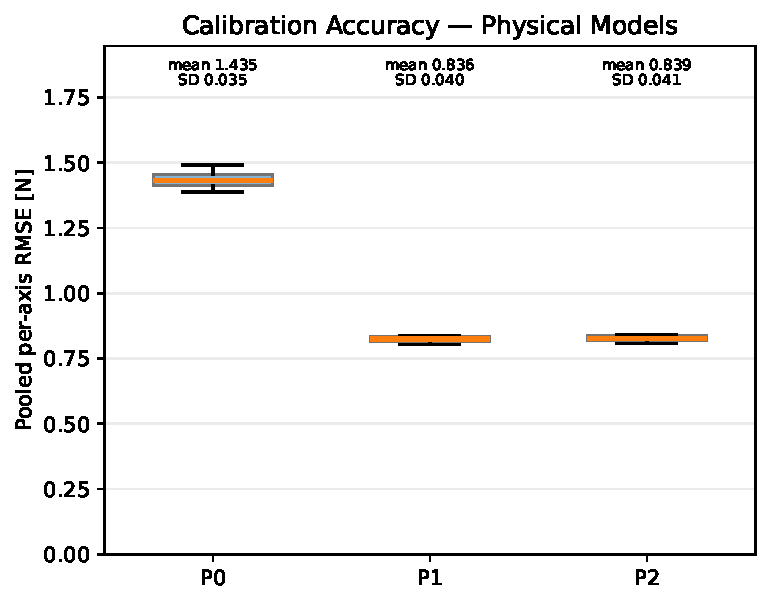
\includegraphics[width=0.82\linewidth]{figures/4_2_accuracy_Physical_Models.pdf}
\caption{Test A pooled force RMSE across remountings.}
\label{fig:4_2_accuracy_Physical_Models}
\end{figure}

\begin{figure}[tb]
\centering
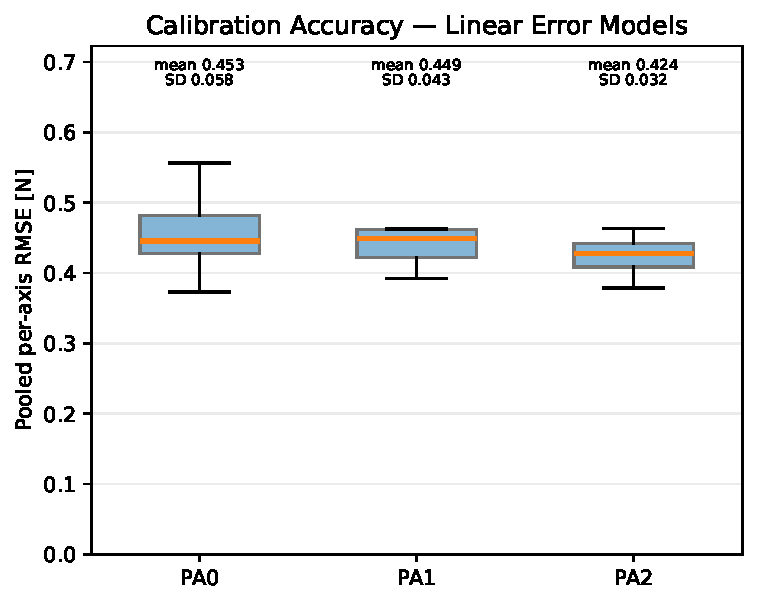
\includegraphics[width=0.82\linewidth]{figures/4_2_accuracy_Linear_Error_Models.pdf}
\caption{Test A pooled force RMSE across remountings.}
\label{fig:4_2_accuracy_Linear_Error_Models}
\end{figure}

\begin{figure}[tb]
\centering
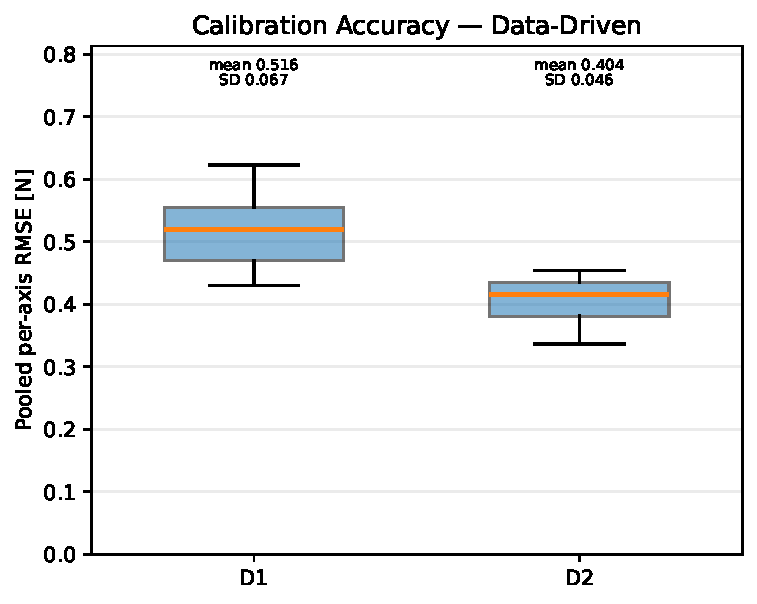
\includegraphics[width=0.82\linewidth]{figures/4_2_accuracy_Data-Driven.pdf}
\caption{Test A pooled force RMSE across remountings.}
\label{fig:4_2_accuracy_Data-Driven}
\end{figure}

\begin{figure}[tb]
\centering
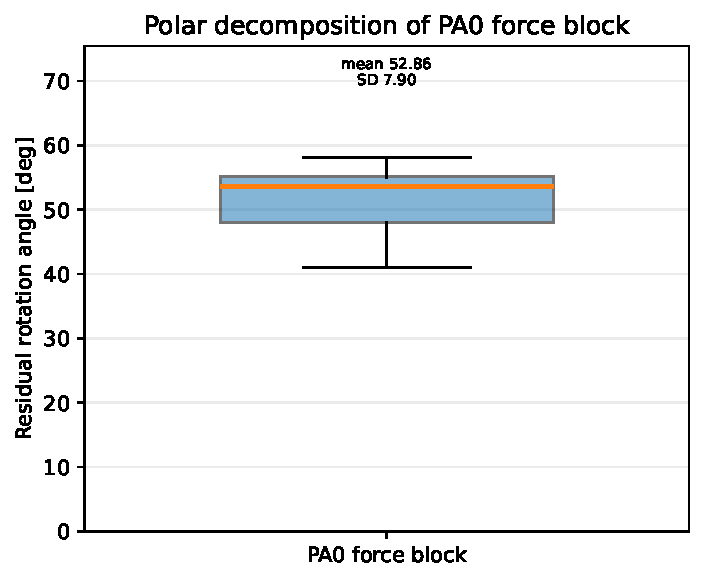
\includegraphics[width=0.82\linewidth]{figures/4_2_pa0_rotation_angle.pdf}
\caption{Residual rotation angle from polar decomposition of the PA0 force-input block.}
\label{fig:pa0_rotation}
\end{figure}

\begin{figure}[tb]
\centering
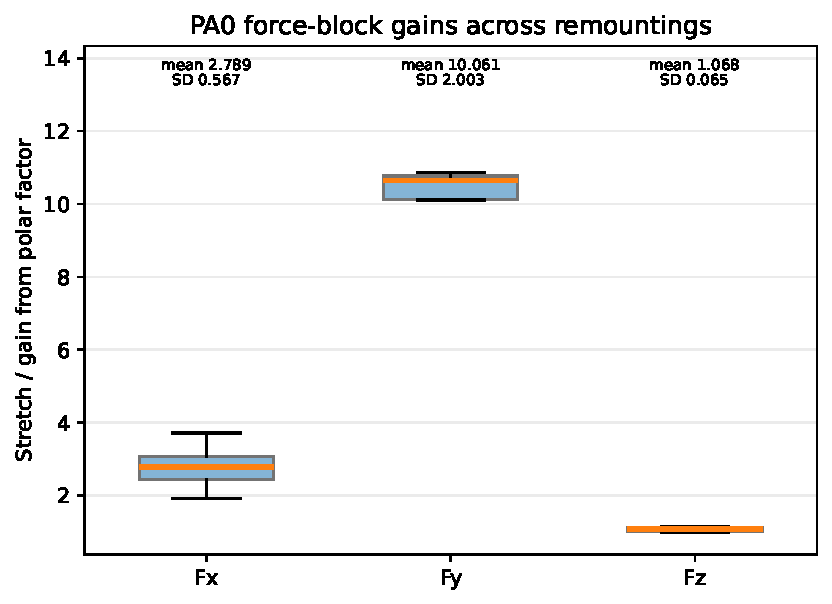
\includegraphics[width=0.82\linewidth]{figures/4_2_pa0_axis_gains.pdf}
\caption{Axis stretch terms from polar decomposition of the PA0 force-input block.}
\label{fig:pa0_gains}
\end{figure}

\begin{figure}[tb]
\centering
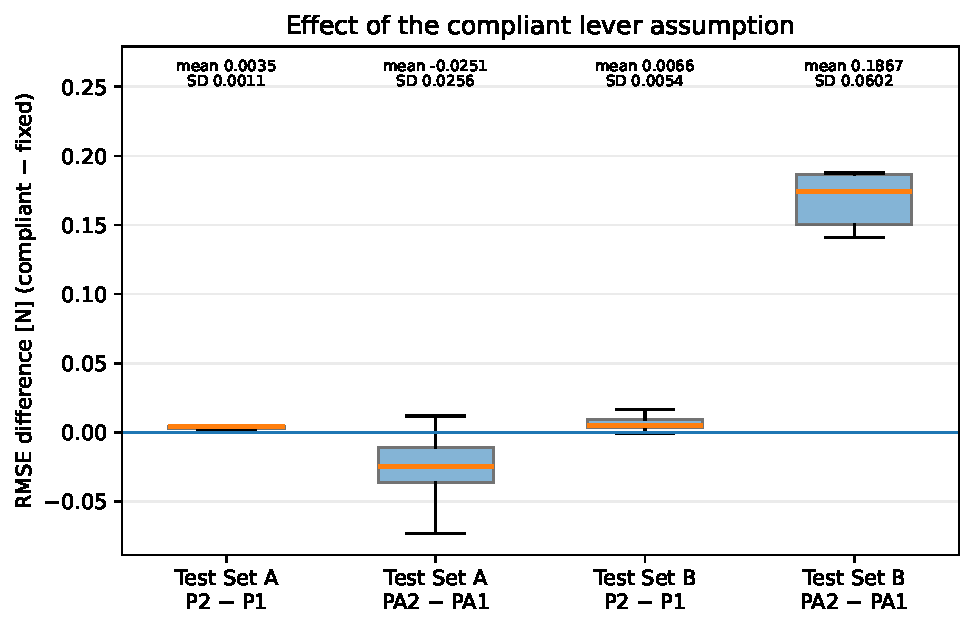
\includegraphics[width=0.82\linewidth]{figures/4_2_compliance_effect.pdf}
\caption{Paired effect of the compliant lever assumption on pooled RMSE.}
\label{fig:compliance_effect}
\end{figure}

\begin{figure}[tb]
\centering
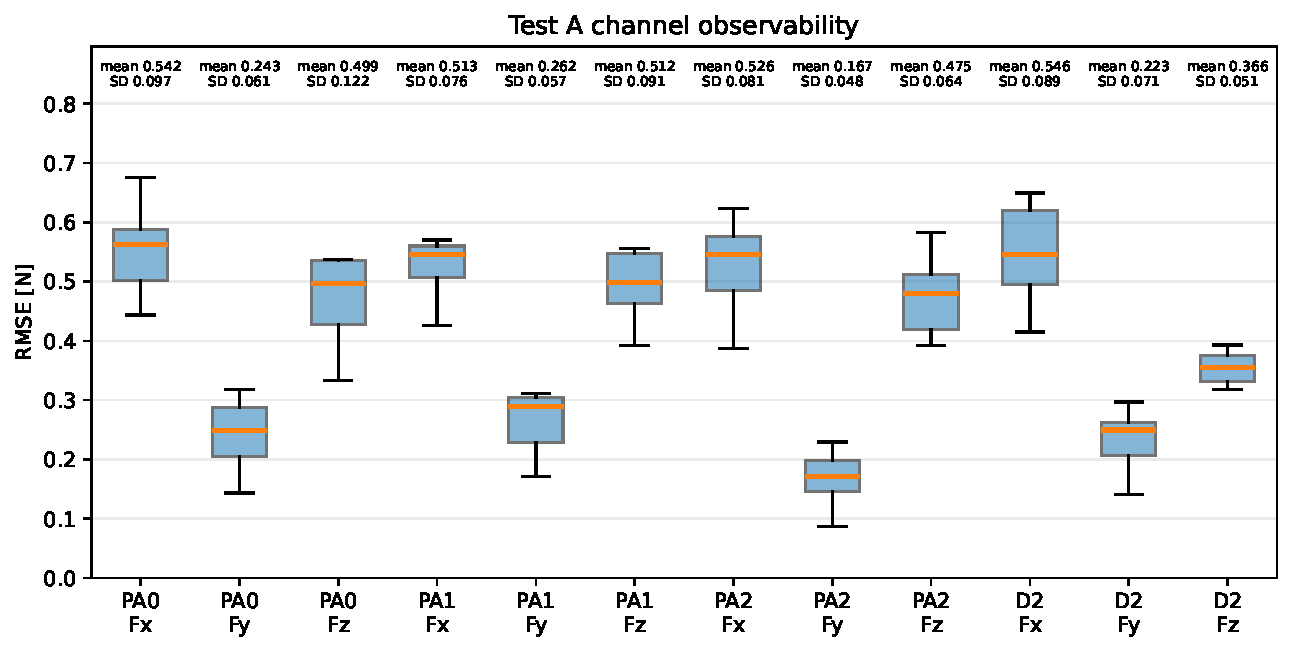
\includegraphics[width=0.82\linewidth]{figures/4_2_channel_rmse.pdf}
\caption{Test A force-channel RMSE for the moment, hybrid and benchmark models.}
\label{fig:channel_rmse}
\end{figure}

\subsection{Independent dead-weight validation}

\begin{figure}[tb]
\centering
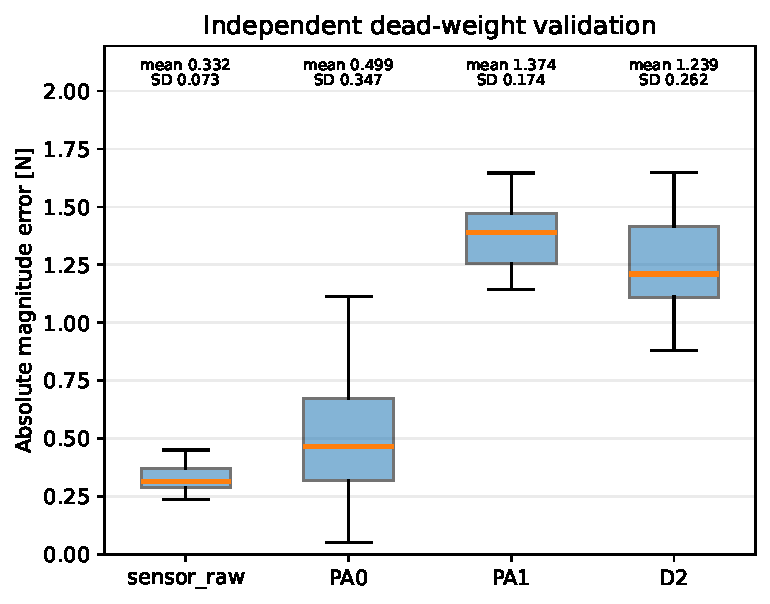
\includegraphics[width=0.82\linewidth]{figures/4_3_deadweight_validation.pdf}
\caption{Independent dead-weight validation.}
\label{fig:deadweight}
\end{figure}

\subsection{Repeatability and remounting}

\begin{figure}[tb]
\centering
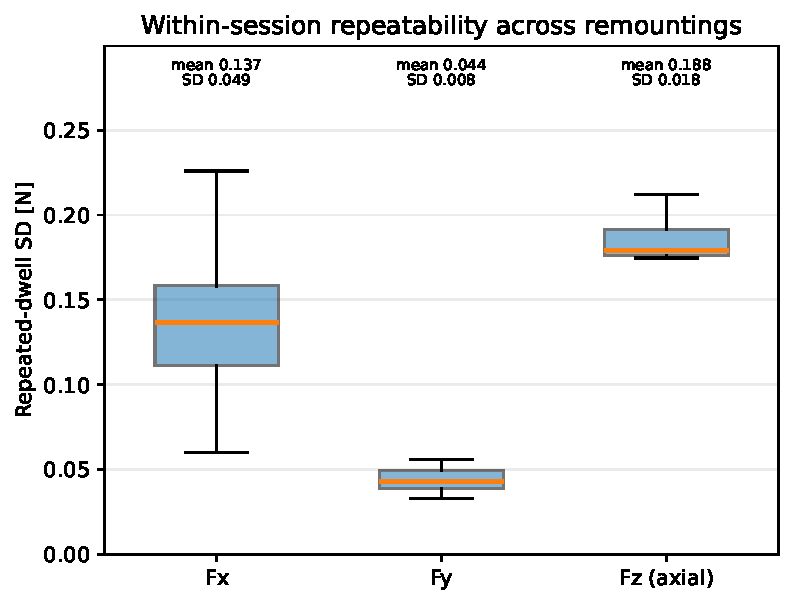
\includegraphics[width=0.82\linewidth]{figures/4_4_repeatability_channels.pdf}
\caption{Within-session repeated-dwell standard deviation by force channel.}
\label{fig:repeatability}
\end{figure}

\begin{figure}[tb]
\centering
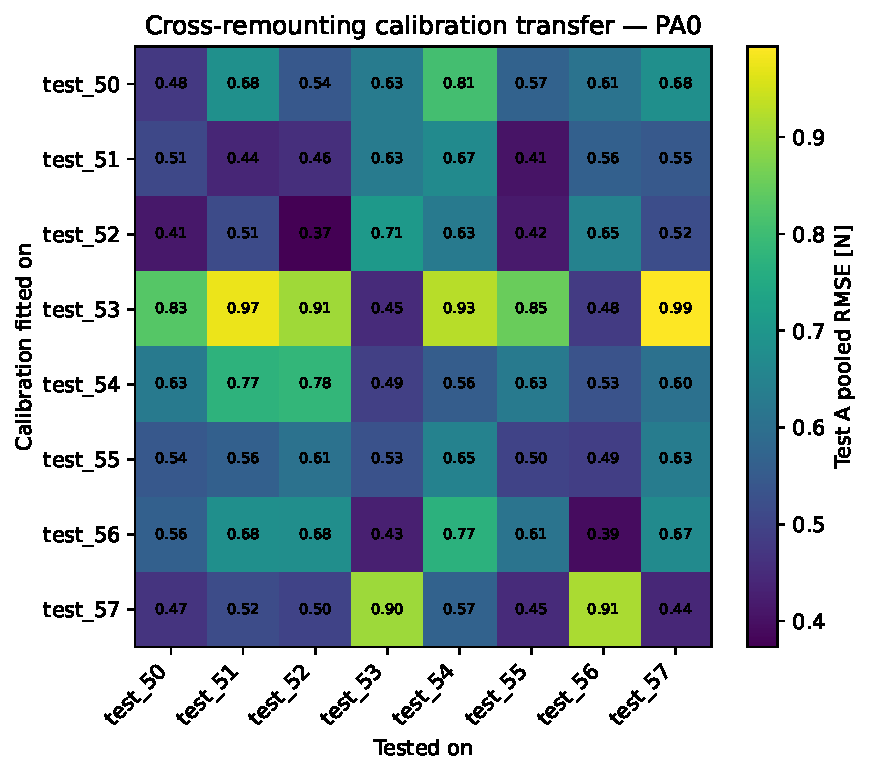
\includegraphics[width=0.82\linewidth]{figures/4_4_transfer_PA0.pdf}
\caption{Cross-remounting transfer matrix for PA0.}
\label{fig:transfer_pa0}
\end{figure}

\subsection{Robustness outside the calibration amplitude}

\begin{figure}[tb]
\centering
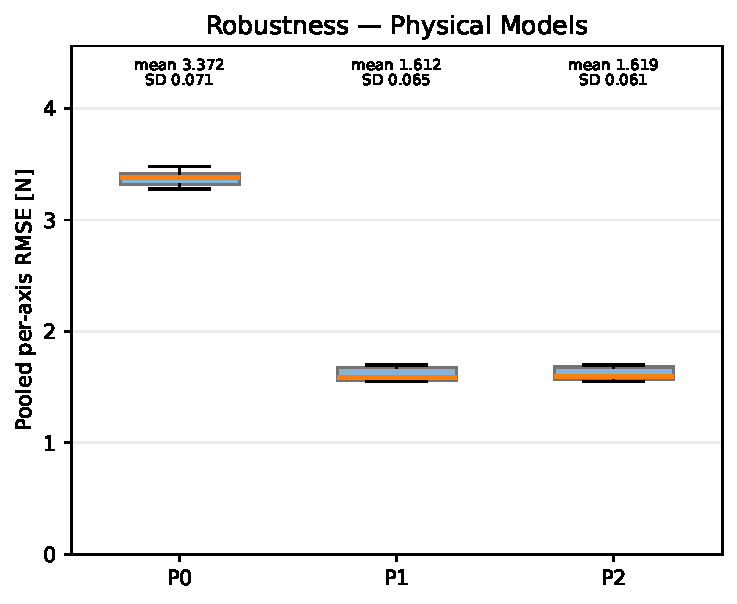
\includegraphics[width=0.82\linewidth]{figures/4_5_robustness_Physical_Models.pdf}
\caption{Test B pooled force RMSE across remountings.}
\label{fig:4_5_robustness_Physical_Models}
\end{figure}

\begin{figure}[tb]
\centering
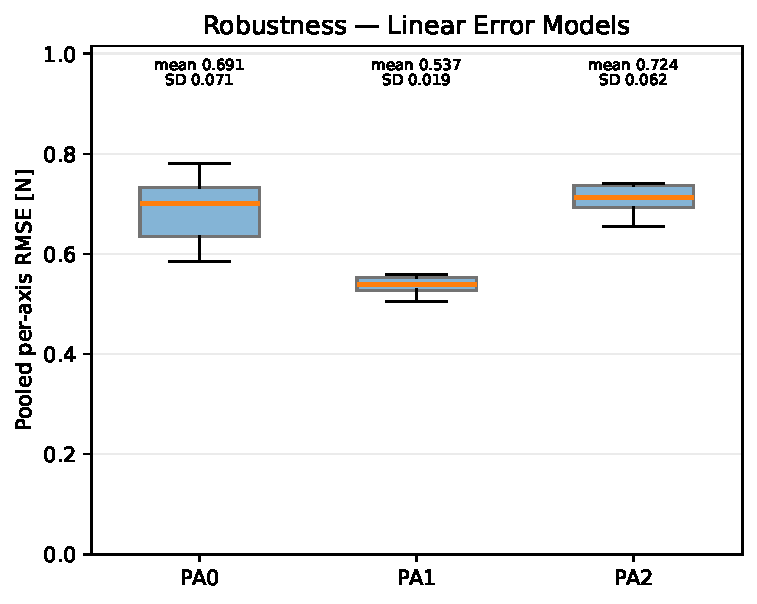
\includegraphics[width=0.82\linewidth]{figures/4_5_robustness_Linear_Error_Models.pdf}
\caption{Test B pooled force RMSE across remountings.}
\label{fig:4_5_robustness_Linear_Error_Models}
\end{figure}

\begin{figure}[tb]
\centering
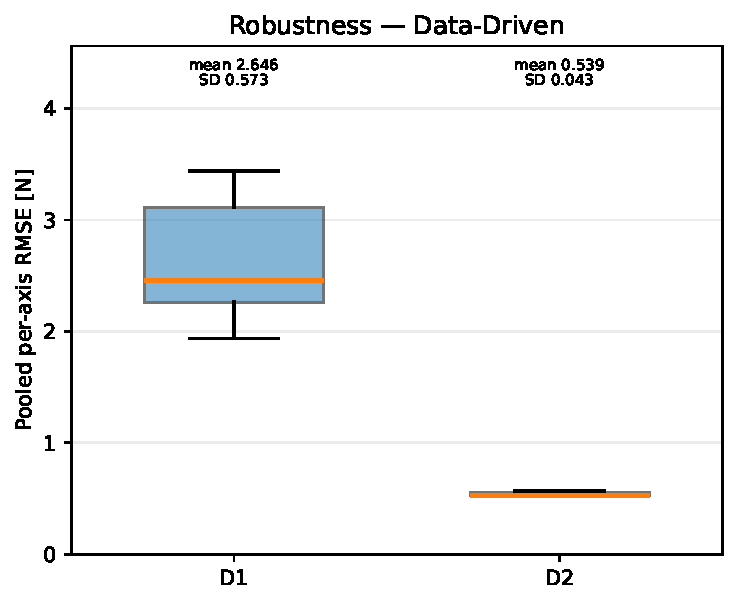
\includegraphics[width=0.82\linewidth]{figures/4_5_robustness_Data-Driven.pdf}
\caption{Test B pooled force RMSE across remountings.}
\label{fig:4_5_robustness_Data-Driven}
\end{figure}

\begin{figure}[tb]
\centering
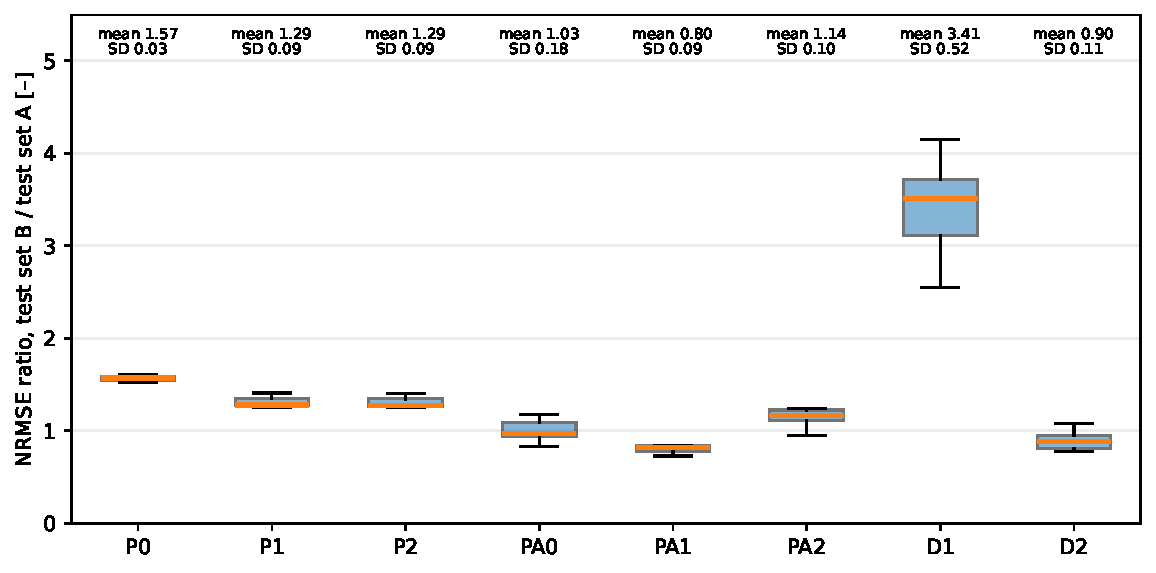
\includegraphics[width=0.82\linewidth]{figures/4_5_degradation.pdf}
\caption{Ratio of normalized RMSE, test set B / test set A, across remountings (normalization loads 4.0 N and 6.0 N).}
\label{fig:degradation}
\end{figure}

\begin{figure}[tb]
\centering
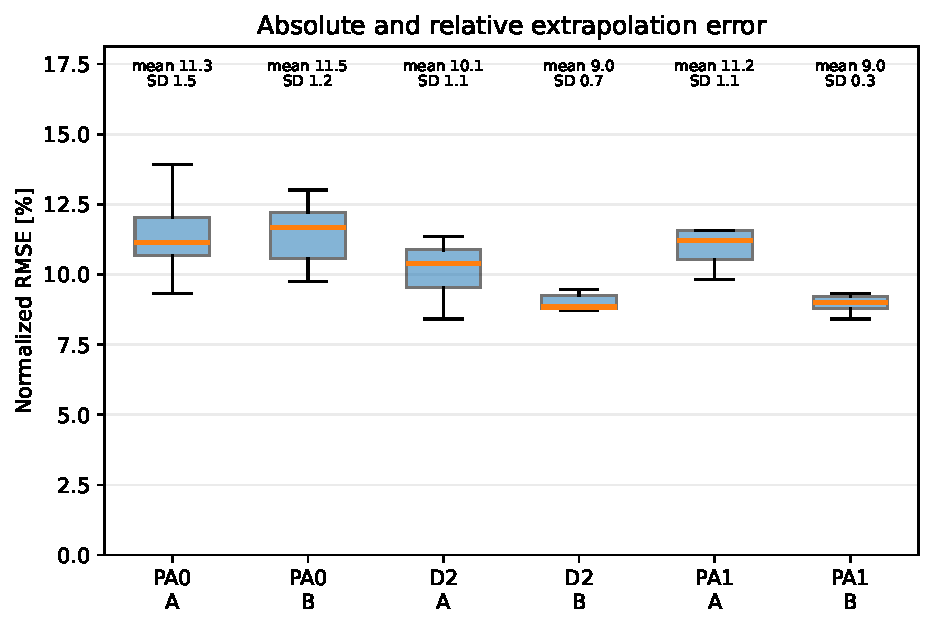
\includegraphics[width=0.82\linewidth]{figures/4_5_normalized_error.pdf}
\caption{Normalized Test A and Test B force error.}
\label{fig:normalized_error}
\end{figure}
